\documentclass[tikz, border=5pt]{standalone}
\usepackage{amsmath, amssymb}
\usetikzlibrary{shapes.geometric, fit, arrows}

\begin{document}
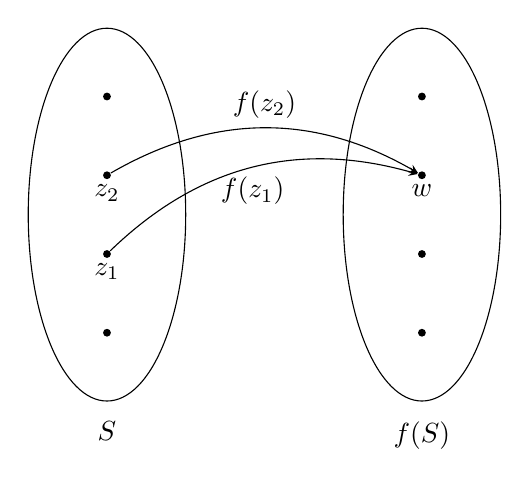
\begin{tikzpicture}[scale=1]
    % define points
    \foreach \x in {1, 2, 3, 4}
    {
        \node[fill, circle, inner sep=1pt] (d\x) at (0, \x) {};
        \node[fill, circle, inner sep=1pt] (r\x) at (4, \x) {};
    }

    % draw ellipses
    \node[fit=(d1) (d4), ellipse, draw, minimum width=2cm] {};
    \node[fit=(r1) (r4), ellipse, draw, minimum width=2cm] {};

    % label ellipses
    \node[below] at (0, 0) {$S$};
    \node[below] at (4, 0) {$f(S)$};

    % point labels
    \node[below] at (d2) {$z_1$};
    \node[below] at (d3) {$z_2$};
    \node[below] at (r3) {$w$};

    % arrows
    \draw[->, >=stealth] (d2) edge[bend left] node[below]{$f(z_1)$} (r3);
    \draw[->, >=stealth] (d3) edge[bend left] node[above]{$f(z_2)$} (r3);
\end{tikzpicture}
\end{document}
